\documentclass[11pt,letterpaper]{article}
%%%%%%%%%%% DOC CLASS & PACKAGES %%%%%%%%%%%%
\usepackage{graphicx,enumerate,amsmath,titlesec,amssymb,microtype,sectsty,float,subcaption}
\usepackage[bottom]{footmisc}

\usepackage[hidelinks]{hyperref}
%\usepackage{hyperref}



%%%%%%%%%%% MARGINS AND SPACING %%%%%%%%%%%%
% Set margins
% \setlength{\topmargin}{-0.5in}
% \setlength{\bottommargin}{-0.5in}
% \setlength{\textheight}{9in}
% \setlength{\textwidth}{6.5in}
% \setlength{\oddsidemargin}{0in}


%\usepackage[left=1.5cm,right=1.5cm,top=2cm,bottom=1cm]{geometry}
\usepackage[left=.75in,right=.75in,top=.75in,bottom=.75in]{geometry}


% Set Paragraph Spacing 
\setlength{\parskip}{0pt}
\setlength{\parindent}{0pt}

% Footnotes - Gap & Force to Bottom
\setlength{\footnotesep}{\baselineskip}
\usepackage[bottom]{footmisc}


%%%%%%%%%%% DOUBLE SPACING %%%%%%%%%%%%
% \usepackage{setspace}
% \doublespacing
% \sectionfont{\MakeUppercase}
% \subsectionfont{\MakeUppercase}



%%%%%%%%%%% FANCY HEADINGS %%%%%%%%%%%%
% \usepackage{fancyhdr}
% \pagestyle{fancy}
% \renewcommand{\headrulewidth}{0.3pt}
% \renewcommand{\footrulewidth}{0.0pt}
% \renewcommand{\sectionmark}[1]{\markboth{#1}{}} % set the \leftmark
% \lhead{\textsc{\nouppercase{\leftmark}}}
% \rhead{\textsc{Right Heading}}
% \cfoot{\thepage}


%%%%%%%%%%% SECTION HEADING FONT %%%%%%%%%%%%
\usepackage[T1]{fontenc}
\sectionfont{\scshape}
\subsectionfont{\scshape}
\subsubsectionfont{\scshape}


%%%%%%%%%%% SANS SERIF %%%%%%%%%%%%
% \usepackage{lmodern}
% \usepackage[T1]{fontenc}
% \usepackage{amsmath,amsthm}
% \usepackage{sansmathfonts}
% \renewcommand{\familydefault}{\sfdefault}


\begin{document}



%%%%%%%%%%% TITLEPAGE %%%%%%%%%%%%%
\begin{center}
  \Huge{\textsc{\textbf{UCSB Controls Lab TA Manual}}}
  \vspace{0.5cm}
  \\ \textbf{\textsc{By} \large{\textsc{Max Crisafulli}}}
  \vspace{0.2cm}
  \\ \textsc{September 2024}

  \vspace{\fill}

\begin{figure}[H]
    \centering
    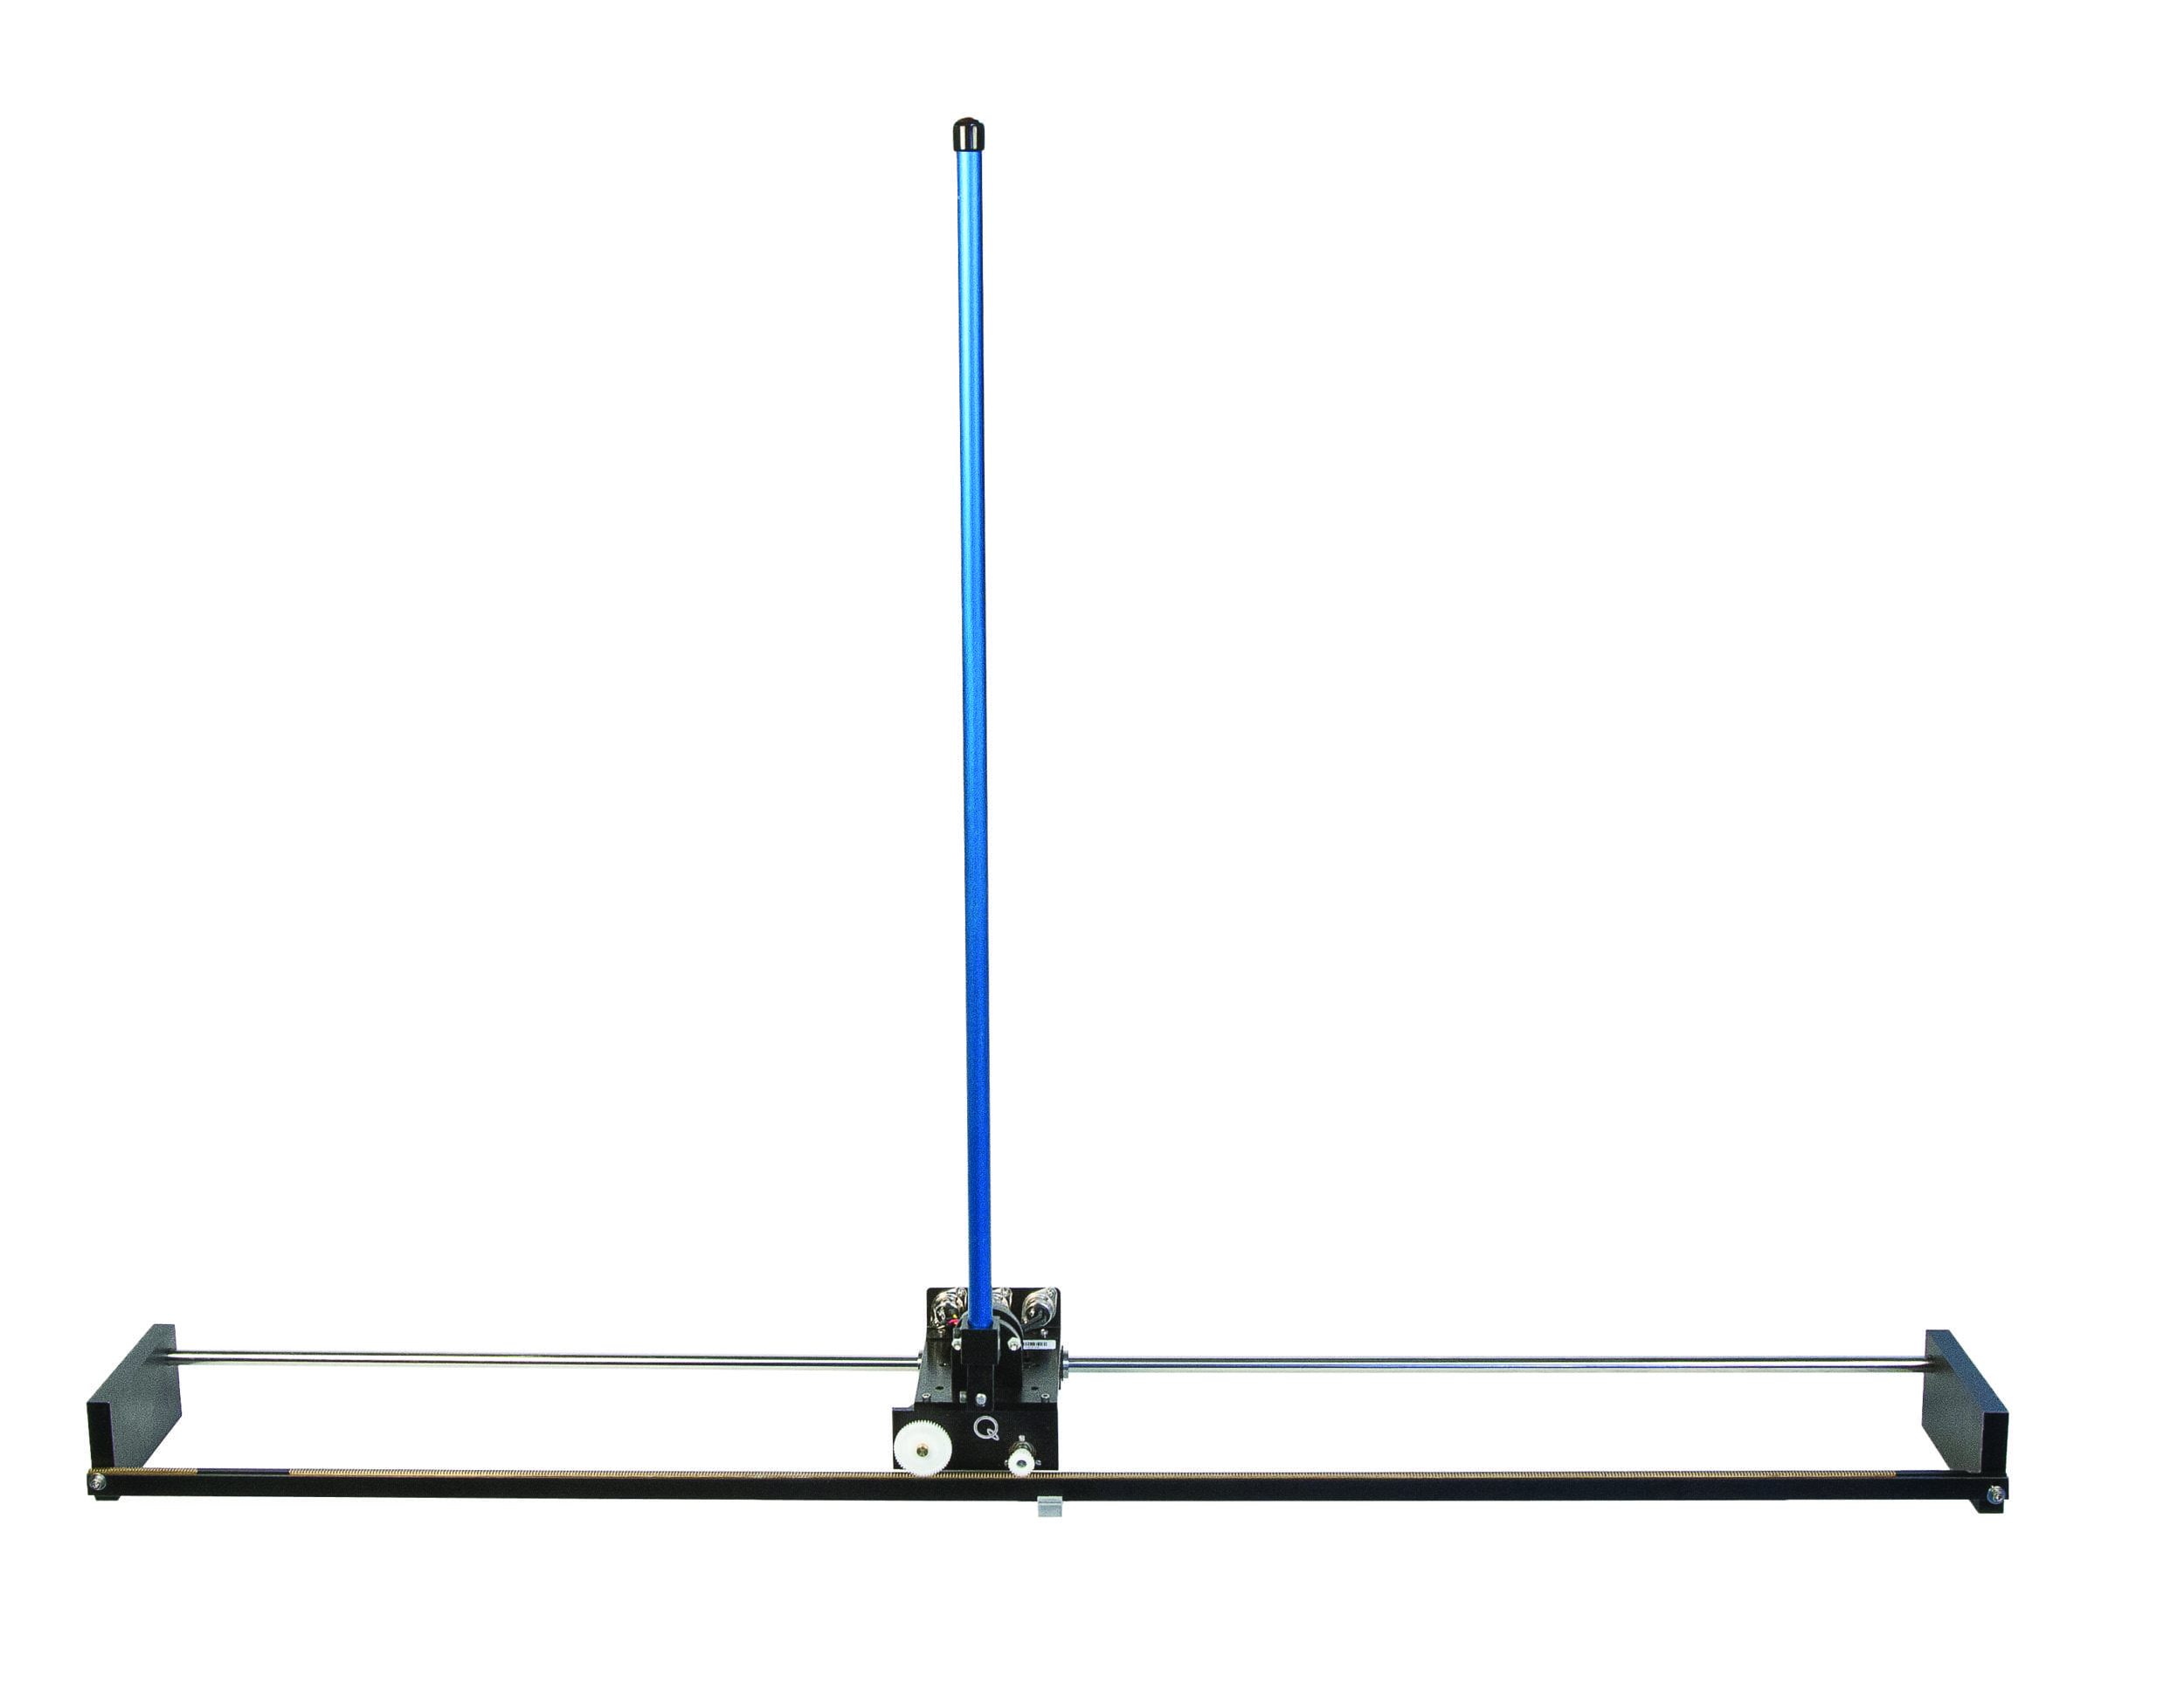
\includegraphics[width=1\textwidth]{./Figures/IP02-Inverted-Pendulum_graphics.jpg}
    % \vspace{-1.75cm}
    % \caption*{Quanser Inverted Pendulum System}
\end{figure}

\vspace{\fill}


\textsc{This document lives at} \\
\url{https://github.com/MaxCrisafulli/UCSB-ControlsLab-Manual-2024}
\end{center}
\thispagestyle{empty}

%%%%%%%%%%% SKIPPED PAGE  %%%%%%%%%%%%%
\newpage
\phantom{}
\thispagestyle{empty}
\newpage
\setcounter{page}{1}


\section*{TA Manual for the UCSB ECE Controls Lab}
This document is to act as a guide for TAs in setting up the Quanser inverted pendulum cart hardware in the UCSB ECE Controls Lab (Harold Frank Hall 3120A). This guide is an update of the existing manual, located at:
\[ \text{ \url{https://github.com/justinpearson/UCSB-Quanser-Inverted-Pendulum-Lab-Manual}}\]
This updated guide will live (and hopefully be maintained) at 
\[\text{\url{https://github.com/MaxCrisafulli/UCSB-ControlsLab-Manual-2024}}\]
\subsection*{Hardware In The Lab}
The ECE147 labs make use of the Quanser `Linear Servo Base Unit with Inverted Pendulum'. This manual will detail the setup of just the cart system, with motor voltage as input and linear position as output. There are 3 main components of the hardware setup, with each of which being explained below.

\subsubsection*{Q4 DAQ Board}
The SIMULINK model that interfaces with the hardware interacts with the world via the Q4 HIL control card and DAQ (Data Acquisition Board). The control card is inside the lab PCs connected via PCIe and interfaces with the DAQ board via the two gray ribbon cables. Ensure that these are connected properly and that the red Status LED is lit, indicating that the board is powered.
\begin{figure}[H]
  \centering
  \includegraphics[width=.75\textwidth]{./Figures/DAQboard_annotated.png}
  \caption{Quanser Q4 Terminal DAQ Board}
\end{figure}
The DAQ board uses the four encoder ports to read signals from the hardware. Generally, Encoder 0 is used for the linear position encoder. In the top left corner of the board are the Analog Outputs, Analog Output 0 is used to drive the amplifier box which ultimately drives the cart motor.



\subsubsection*{VoltPAQ-X1 Amplifier}
The Quanser VoltPAQ-X1 Amplifier is powered from a standard wall socket, and turned on via a switch at the back of the box. Make sure that the green status LED in the center of the amplifier diagram is lit, indicating that the amplifier is powered on. Also check that the Amplifier Gain switch is set to 1x.


\begin{figure}[H]
  \centering
  \includegraphics[width=.75\textwidth]{./Figures/amplifier_annotated.png}
  \caption{Quanser VoltPAQ-X1 Linear Voltage Amplifier}
\end{figure}

The red AV cable coming from Analog Output 0 on the DAQ board should be connected to the Amplifier Command (input) port. The white AV cable should be connected to Current Sense on the amplifier and Analog Input 0 on the DAQ board, although this is not necessary. \\

The output of the amplifier (To Load) is what drives the motor onboard the cart. Check that all the cable connections are correct and that the cable going to the motor has enough slack to allow the cart to move along the track. 

\subsubsection*{Inverted Pendulum Cart System}
The cart system has 2 encoder outputs and 1 analog voltage input. The positions of these ports may vary between the carts but in general they are as depicted in Figure \ref{fig:cart}. You should check what each of the ports connect to before plugging anything in. \\

The cart controls its position along the track with the smaller motor drive wheel, which is driven by the motor voltage coming from the amplifier. The larger position encoder wheel measures the relative position along the track from the time that the program was initialized in `ticks'. The conversion ratio from ticks to inches is approximately 5000 ticks per 6 inches.
\begin{figure}[H]
  \centering
  \includegraphics[width=.75\textwidth]{./Figures/cart_annotated.png}
  \caption{Quanser Linear Servo Base Unit (The `Cart')}
  \label{fig:cart}
\end{figure}



\subsection*{Instructions}
The following slides will detail setting up a minimum working SIMULINK model that can pass a voltage to the motor and read position from the cart encoder.

\end{document}